\begin{table*}[t]
\begin{picture}(\linewidth, 0.625\linewidth)
\put(0, 98){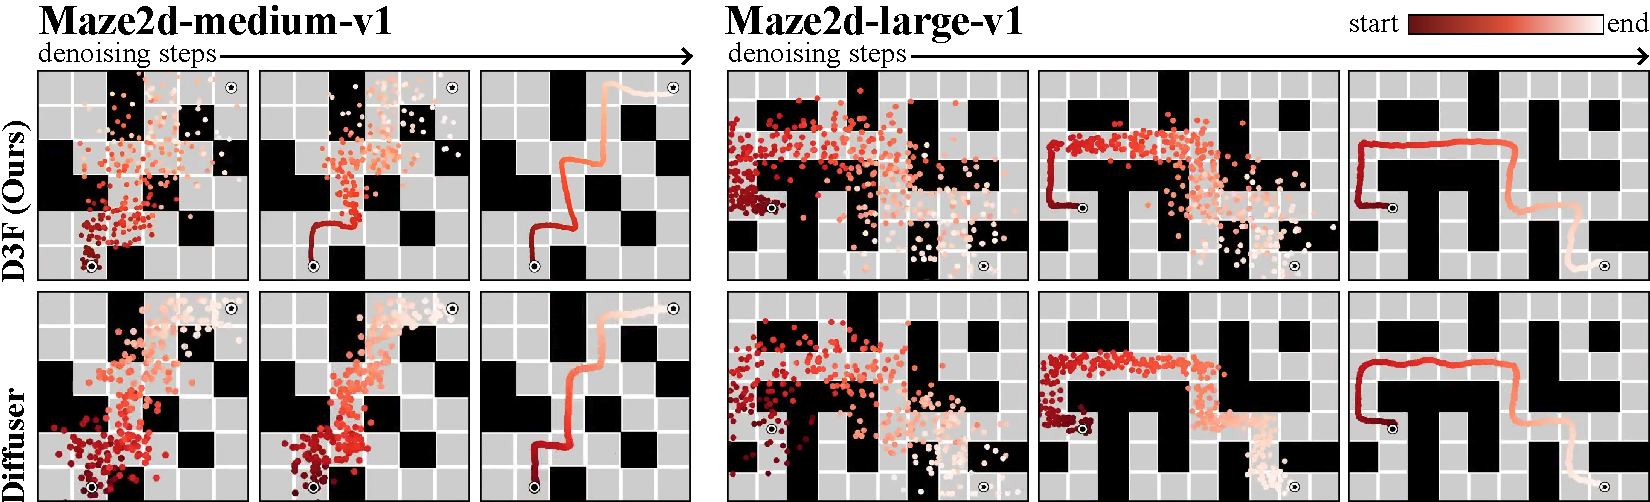
\includegraphics[width=\linewidth]{figures/pdf/Maze.pdf} }
\put(0, 43){
\resizebox{\linewidth}{!}{%
\begin{tabular}{@{}llccccccc@{}}
    \FL
    \multicolumn{2}{c}{\textbf{Environment}} & \textbf{MPPI} & \textbf{CQL} & \textbf{IQL} & \textbf{Diffuser*} & \textbf{Diffuser w/ diffused action} & \textbf{Ours wo/ MCG} & \textbf{Ours}\ML
    Maze2D & U-Maze & 33.2 & 5.7 & 47.4 & 113.9 \(\pm\) 3.1 & 6.3 \(\pm\) 2.1& 110.1 \(\pm\) 3.9 & \textbf{116.7 \(\pm\) 2.0} \NN
    Maze2D & Medium & 10.2 & 5.0 & 34.9 & 121.5 \(\pm\) 2.7 & 13.5\(\pm\)2.3 & 136.1 \(\pm\) 10.2 & \textbf{149.4 \(\pm\) 7.5} \NN
    Maze2D & Large & 5.1 & 12.5 & 58.6 & 123.0 \(\pm\) 6.4 & 6.3 \(\pm\)2.1 & 142.8 \(\pm\) 5.6 & \textbf{159.0 \(\pm\) 2.7} \ML
    \multicolumn{2}{c}{\textbf{Single-task Average}} & 16.2 & 7.7 & 47.0 & 119.5 & 8.7 & 129.67 & \textbf{141.7}  \ML[0.11em]
    Multi2D & U-Maze & 41.2 & - & 24.8 & 128.9 \(\pm\) 1.8 & 32.8\(\pm\)1.7 & 107.7 \(\pm\) 4.9 & \textbf{119.1 \(\pm\) 4.0} \NN
    Multi2D & Medium & 15.4 & - & 12.1 & 127.2 \(\pm\) 3.4 & 22.0\(\pm\)2.7 & 145.6 \(\pm\) 6.5 & \textbf{152.3 \(\pm\) 9.9} \NN
    Multi2D & Large & 8.0 & - & 13.9 & 132.1 \(\pm\) 5.8 & 6.9 \(\pm\)1.7 & 129.8 \(\pm\) 1.5 & \textbf{167.1 \(\pm\)2.7}  \ML
    \multicolumn{2}{c}{\textbf{Multi-task Average}} & 21.5 & - & 16.9 & 129.4 & 20.6 &  127.7 & \textbf{146.2} \LL
\end{tabular}
}
}
\end{picture}

\caption{ \textbf{\algons{} for Planning.} (\textbf{top}) During sampling, \algo{} allows each time step to be denoised on different noise schedules, enabling us to account for causal uncertainty during guided planning. \algo{} keeps the far future more uncertain than the near future while Diffuser~\cite{janner2022planning} puts them at the same noise level during sampling. (\textbf{bottom)} Quantitatively, \algo{} achieves the highest average reward across runs. Diffuser fails dramatically when executing the actually generated actions, requiring a hand-crafted PD controller (indicated by the asterisk) and ignoring generated actions.}
\vspace{-10pt}
\label{fig:planning}
\end{table*}


